% !TEX encoding = UTF-8
% !TEX TS-program = pdflatex
% !TEX root = ../tesi.tex
% !TEX spellcheck = it-IT

%**************************************************************
\chapter{Valutazione retrospettiva}
\label{cap:conclusioni}
Questo capitolo presenta le attività svolte, analizzando se il prodotto sviluppato soddisfa gli obiettivi prefissati. Inoltre, descrivo le problematiche incontrate oltre che un bilancio formativo.
%**************************************************************

%**************************************************************

%**************************************************************
\section{Bilancio sui risultati}

\subsection{Obiettivi soddisfatti}
Gli obiettivi prefissati prima dell'inizio dello stage hanno subito delle leggere modifiche, dovute principalmente alla strategia aziendale, privilegiando lo sviluppo del nuovo modulo \textit{Tres}. Infatti il \textit{porting} del modulo \textit{Dre} non è stato ultimato, ad eccezione di un'unica attività, quella del \textit{map reduce}. Questo ha comportato il mancato sviluppo di nuovi algoritmi, mancando di conseguenza gli obiettivi massimi prefissati, che riguardavano principalmente l'introduzione di nuovi algoritmi di \textit{cluster} per il raggruppamento degli elementi omogenei in un insieme di dati. In seguito a questa aggiunta, avrei dovuto studiare i limiti delle funzioni di apprendimento automatico in modo da introdurre nuovi algoritmi per il miglioramento dello stesso.
Ho soddisfatto invece gli obiettivi minimi che sono da considerare essenziali.\\
Dalle attività di analisi sono riuscito ad individuare 23 requisiti di cui 3 desiderabili. Rispetto al totale, ho soddisfatto l'87\% dei requisiti. Se da un lato i requisiti desiderabili relativi al nuovo modulo non sono stati soddisfatti, dall'altro i requisiti obbligatori sono stati tutti soddisfatti.\\


 I requisiti non soddisfatti riguardano gli obiettivi massimi di implementazione di nuovi algoritmi di apprendimento.
 
 
\begin{figure}[h]
\centering
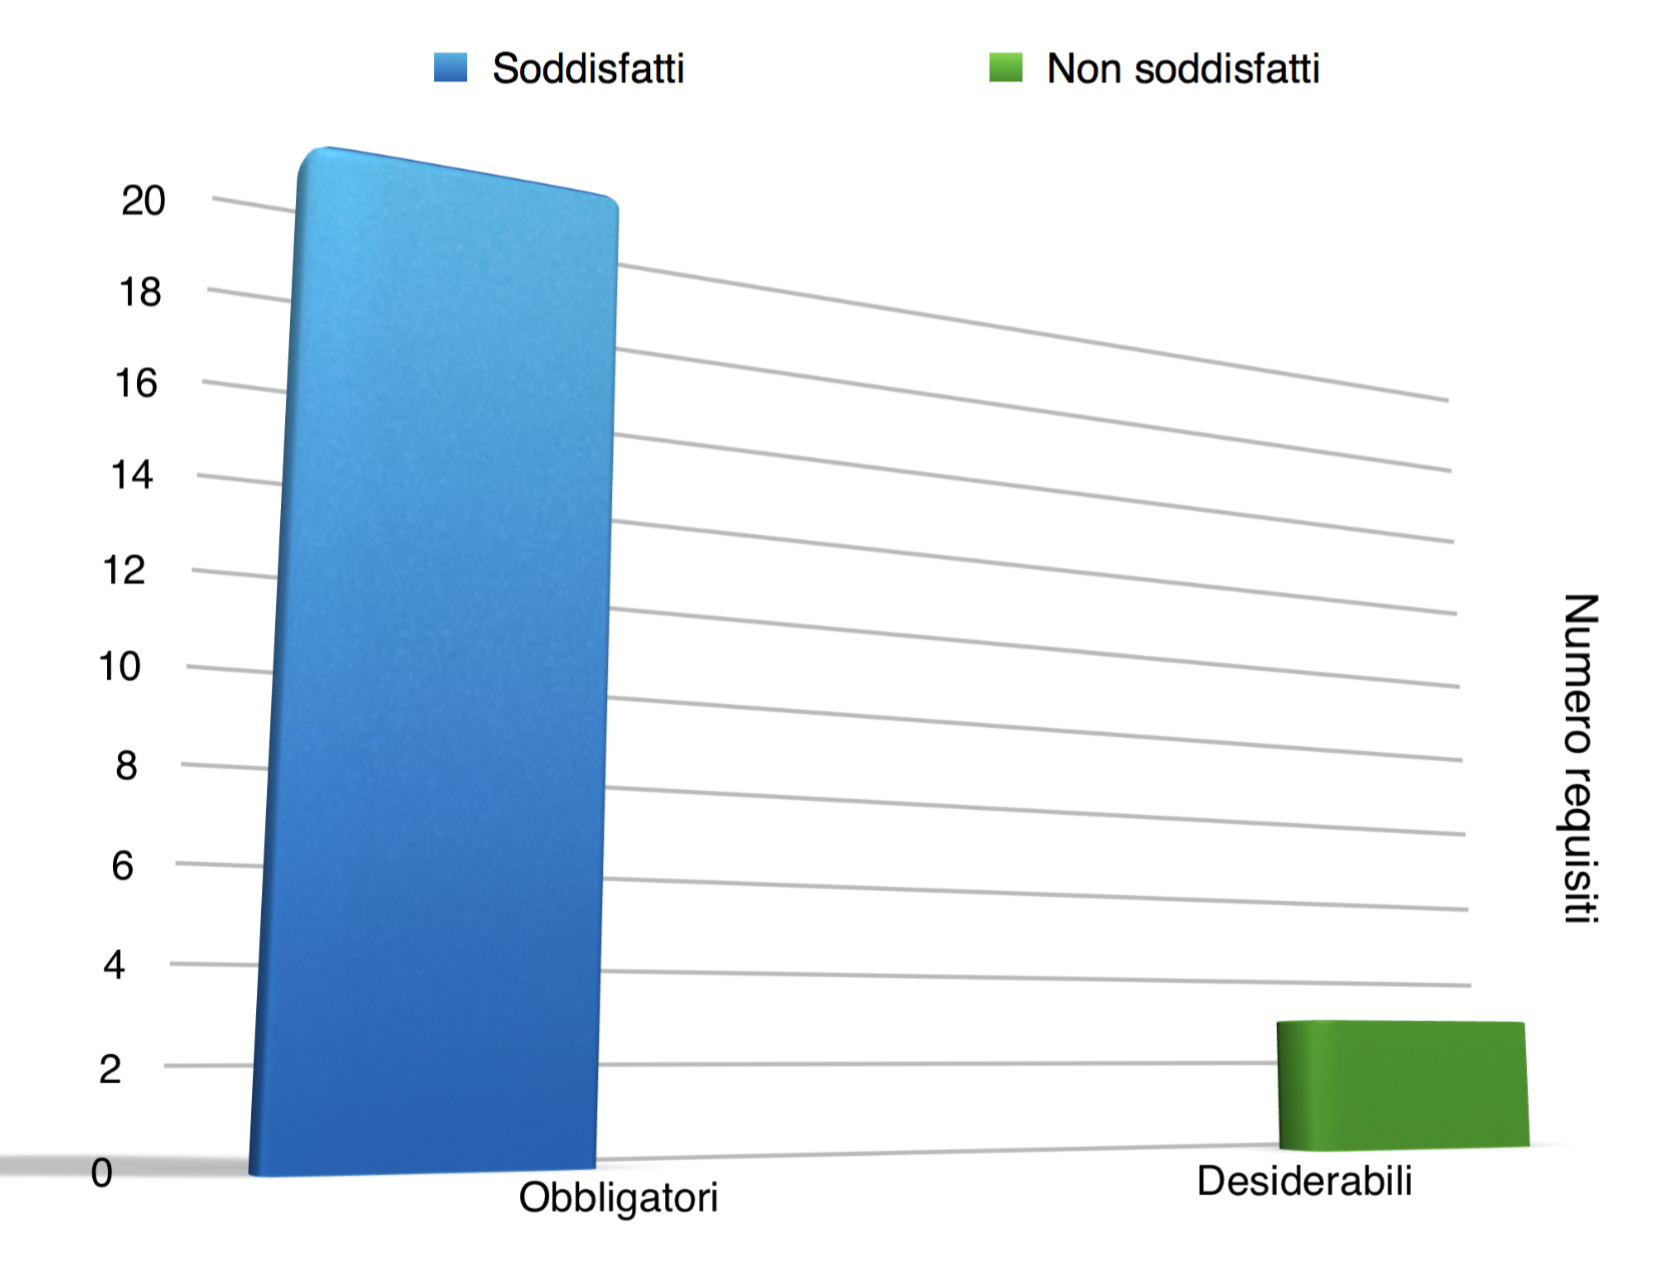
\includegraphics[width=0.7\linewidth]{immagini/chartReq}
\caption[Rappresentazione requisiti]{Rappresentazione requisiti}
\label{fig:chartReq}
\end{figure}

\newpage
Il sistema da me realizzato supporta al momento l'estrazione di informazioni utili al supporto delle decisioni. Le funzionalità attuali sono una buona base per sviluppi futuri.

\subsection{Obiettivi personali} 
Il mio obiettivo di lavorare con tecnologie del \textit{Data Mining}, di esplorare e di modellare grandi masse di dati è stato dunque raggiunto. Attraverso questo progetto sono riuscito ad avere un'introduzione ai \textit{big data}, che sono sicuramente uno dei temi più caldi nel panorama tecnologico attuale. Anche l'interesse da parte delle aziende è alto, consapevoli del patrimonio di dati in loro possesso e dei vantaggi strategici in termini di business attraverso una corretta gestione dei dati. \\


\section{Problematiche riscontrate}
Dato che lo stage è un'occasione di conoscenza diretta con il mondo del lavoro, oltre che di acquisizione di nuove conoscenze, ho dovuto scontrarmi con tecnologie, strumenti e modalità di lavoro a me nuovi. 
\subsection*{Pianificazione attività}
Durante la pianificazione ho sottostimato l'attività di studio. Il ritardo è dovuto alla durata delle video-lezioni del linguaggio Scala, tutorial consigliato dal responsabile che ho seguito in modo da apprenderlo nel suo paradigma funzionale. Ho dovuto quindi recuperare le ore dalle altre attività nelle quali avevo previsto un periodo di \textit{slack}.

\subsection*{Sviluppare con Scala}
La difficoltà iniziale è stato cambiare lo stile di programmazione imperativo a uno stile funzionale.
Particolarmente ardua è stata l'adozione delle funzioni \textit{curry}. Questa metodologia trasforma una funzione che accetta più argomenti in una catena di funzioni ognuna delle quali accetta un singolo argomento. Le funzioni \textit{curry} vengono definite con molteplici liste di parametri. La principale difficoltà stava nella leggibilità della sintassi. Un altro problema è stato l'interfacciamento al \textit{database}, dove ho dovuto utilizzare il \textit{pattern matching} cioè la possibilità di compiere scelte programmatiche tra molteplici condizioni. Alla fine, l'utilizzo di queste funzionalità si è rivelato molto semplice anche se a prima vista mi è sembrato difficoltoso.

\subsection*{Analisi dei requisiti}
Durante l'attività di analisi ho avuto non pochi problemi a capire le funzionalità dell'applicativo da sviluppare. Anche se le riunioni non mancavano, ho avuto una difficoltà iniziale a interagire e arrivare a un accordo con il responsabile sui requisiti da implementare. La difficoltà è salita quando è intervenuto il \textit{CEO} con concetti diversi rispetto a lui. La situazione è rimasta in stallo per alcuni giorni, ma dopo numerosi incontri sono arrivato a una soluzione e i requisiti identificati sono stati accettati. La sua conferma mi ha permesso di procedere con la progettazione.



%**************************************************************

\section{Bilancio formativo}

\subsection{Competenze acquisite}
Lo stage mi ha permesso di lavorare con tecnologie nuove e innovative del \textit{data mining e machine learning}, un campo molto caldo che sta avendo molto successo. Ovviamente, il mio bagaglio di conoscenze si è arricchito con le seguenti tecnologie:

	\subsection*{Scala}  
	Scala mi ha permesso di utilizzare la programmazione funzionale, un paradigma mai usato in precedenza con il quale ho avuto delle difficoltà iniziali, ma i punti a favore sono tanti. In primo luogo, il più importante, a mio avviso, riguarda le collezioni e il modo molto semplice in cui si gestiscono i valori all'interno con funzioni del tipo zip, filter, map che fanno rispettivamente l'unione, filtraggio e il map dei valori di una o più collezioni . Rispetto agli altri linguaggi di programmazione con cui ho lavorato, dove operare su collezioni porta a un codice verboso e contro-intuitivo, Scala offre funzionalità che porta a essere più conciso ed elegante. In secondo luogo, una proprietà importante sono le variabili immutabili che consentono maggiore scalabilità e sicurezza. Questa caratteristica riduce il rischio di inserire bug all'interno del software. Un vantaggio importante è il risparmio di tempo che si può ottenere utilizzando questo linguaggio, per esempio non preoccupandosi più della separazione delle istruzioni oppure della dichiarazione dei \textit{getters e setters} in quanto sono impliciti. Non sono riuscito a usare tutte le funzionalità del linguaggio ma sono contento di aver sperimentato alcuni dei vantaggi derivanti dalla programmazione funzionale. Tornerò sicuramente sul linguaggio per approfondire le mie conoscenze.
	
	\subsection*{Play Framework}
	L'apprendimento di Play non è stato particolarmente difficile. Esso permette di creare in maniera molto semplice un'applicazione. Infatti, Play si occupa di creare e configurare l'applicazione, fornendo una struttura di default. Inoltre, è possibile utilizzare sia il linguaggio Java che Scala. Durante la creazione del \textit{Piano di Lavoro} ero indeciso tra i due linguaggi, per poi scegliere Scala principalmente perché avevo già affrontato Java nel corso di \textit{Programmazione Concorrente e Distribuita} e volevo introdurmi alla programmazione funzionale.
	
	\subsection*{Web Service REStful}
	 Anche se avevo già avuto esperienze con lo stile architetturale \gls{REST}, il progetto mi ha permesso di approfondire le mie conoscenze. Scrivere servizi \gls{REST} in Play framework è molto semplice. Viene utilizzato il \textit{file route} per scrivere le richieste conformi all'approccio \gls{REST} e la richiesta viene associata a un set di istruzioni ben precise nel \textit{controller}.\\ 
	 
	Inoltre, ho usato \gls{JSON}, uno dei più popolari formati per lo scambio di dati.

	\subsection*{OrientDB} 
	OrientDB è un \textit{database} molto flessibile che offre una moltitudine di modalità operative, alcune delle quali anche su strutture a grafo. L'apprendimento, rispetto alle mie esperienze, non è stato difficile. Infatti, OrientDB è uno dei più intuitivi in quanto i nodi sono gli oggetti e gli archi le relazioni tra oggetti. Per questo motivo il \textit{database} non è adatto a ogni soluzione implementativa, ma si presta bene ai domini in cui le entità e le relazioni tra esse possano essere ben espresse come nel caso del mio progetto.

%**************************************************************
\subsection{Valutazione personale}
L'esperienza di stage mi ha permesso di conoscere da vicino un mondo a me prima sconosciuto, quello del lavoro. È stata un esperienza interessante e positiva e ritengo sia essenziale affrontarla prima della conclusione del corso di laurea. Inoltre, mi ha portato ad usare tecnologie mai studiate durante la carriera universitaria. Il corso di laurea fornisce gli strumenti necessari affinché si possano affrontare e apprendere nuove tecnologie. \\
Lo stage mi ha permesso di applicare gli insegnamenti del corso di \textit{Ingegneria del Software}, utilizzando fondamenti e principi durante le differenti fasi dello sviluppo del software. Credo comunque che alcune nozioni, come quelle dei \textit{design pattern} e strumenti di gestione progetto, andrebbero studiati e utilizzati già dal secondo anno per i vari progetti accademici come quello di \textit{Programmazione ad Oggetti} oppure \textit{Tecweb}, il quale si deve fare in gruppo da 4 persone.
\\
L'apprendimento durante il corso degli studi arriva in maniera graduale con il primo grande test, quello di \textit{Programmazione} del primo anno, dove si imparano le basi e comunque la logica che sta dietro a una buona programmazione, con un occhio di riguardo verso la correttezza, alla leggibilità del codice scritto e sopratutto all'ottimizzazione. 
Un altro corso di fondamentale importanza è stato quello di \textit{Programmazione ad Oggetti}, che mi ha permesso di apprendere in modo approfondito la programmazione orientata agli oggetti e di sviluppare una delle prime interfacce grafiche usando le librerie grafiche. Il corso permette di riutilizzare i concetti base della programmazione ad oggetti e trasporli in ambienti diversi dal linguaggio di programmazione C++.\\
Il corso che invece dovrebbe essere aggiornato è \textit{Tecnologie Web}. Il \textit{gap} tecnologico si avverte soprattutto nel guardare le tecnologie che si usano al giorno d'oggi per lo sviluppo di applicazioni web.\\
Penso che il percorso di studi sia completo e offre una preparazione adeguata per affrontare il mondo del lavoro. Uno dei punti fondamentali che mi portano a dire questo, è lo sviluppo del progetto accademico di \textit{Ingegneria del Software} e l'obbligo di \textit{stage}.\\
Ritenendomi soddisfatto dalla formazione ricevuta, entrerò nel mondo del lavoro contento del percorso seguito.
